% !TEX root = main.tex
\section{Introduction}
\subsection{Requirements}
\begin{mytitle}[New Requirements in SW-Technology] These requirements are not satisfied in imperative languages like C, Pascal, Fortran, $\hdots$ \hfill
    \begin{itemize}
        \item Reuse: Quality, Documented Interfaces, Extendibility and Adaptability
        \item Computation as Simulation: Modeling Entities of the Real World, Describing Dynamic System Behaviour, Running Simulations
        \item GUIs: Adaptable Standard Functionality, Concurrency
        \item Distributed Programming: Concurrency, Communication, Distribution of Data and Code
    \end{itemize}
\end{mytitle}
\begin{mytitle}[Core Requirements]\hfill
\begin{itemize}
    \item Cooperating Program Parts with Well-Defined Interfaces: Objects (data and code), Interfaces, Encapsulation
    \item Classification and Specialization: Classification, Subtyping, Polymorphism, Substitution principle
    \item Highly Dynamic Execution Model: Active objects, Message passing
    \item Correctness: Interfaces, Encapsulation, Simple powerful concepts
\end{itemize}
\end{mytitle}

\subsection{Core Concepts}
\begin{mytitle}[The Object Model] A software system is a set of cooperating objects. Objects have state and processing ability. Objects exchange messages.
\begin{center}
    \begin{tabular}{R{0.4\textwidth}|L{0.4\textwidth}}
        Objects & Values \\
        \hline
        State & Can't change state\\
        Identity & Don't have identity\\
        Lifecycle & Don't need to initialize\\
        Location & Don't have a location
    \end{tabular}
\end{center}
\end{mytitle}
\begin{mytitle}[Interfaces and Encapsulation] Objects have well-defined interfaces (publicly accessible fields and methods). Implementation is hidden behind the interface. The interfaces are the basis for describing behaviour.
\end{mytitle}
\begin{mytitle}[Classification and Polymorphism]\hfill
\begin{itemize}
    \item Classification: Hierarchical structuring of objects. Objects belong to different classes simultaneously
    \item Substitution principle: Subtype objects can be used wherever supertype objects are expected.
    \item Polymorphism: A program part is polymorphic if it can be used for objects of several classes.
    \item Subtype polymorphism: A direct consequence of the substitution principle. Program parts working with supertype objects work as well with subtype objects.
    \item Other forms of polymorphism (These are not core concepts): Parametric polymorphism (generic types), Ad-hoc polymorphism (method overloading)
\end{itemize}
\end{mytitle}
\begin{mytitle}[Specialization] Adding specific properties to an object or refining a concept by adding further characteristics. Requires the behaviour of the specialized object to be compliant to the behaviour of more general objects. Program parts that work for the more general objects work as well for specialized objects.
\end{mytitle}
\begin{mytitle}[Summary] Core concepts are abstract concepts to meet the new requirements. To apply the core concepts we need ways to express them in programs. Language concepts enable and facilitate the application of the core concepts.
\end{mytitle}

\subsection{Language Concepts}
Appropriate language support is needed to apply object-oriented concepts.

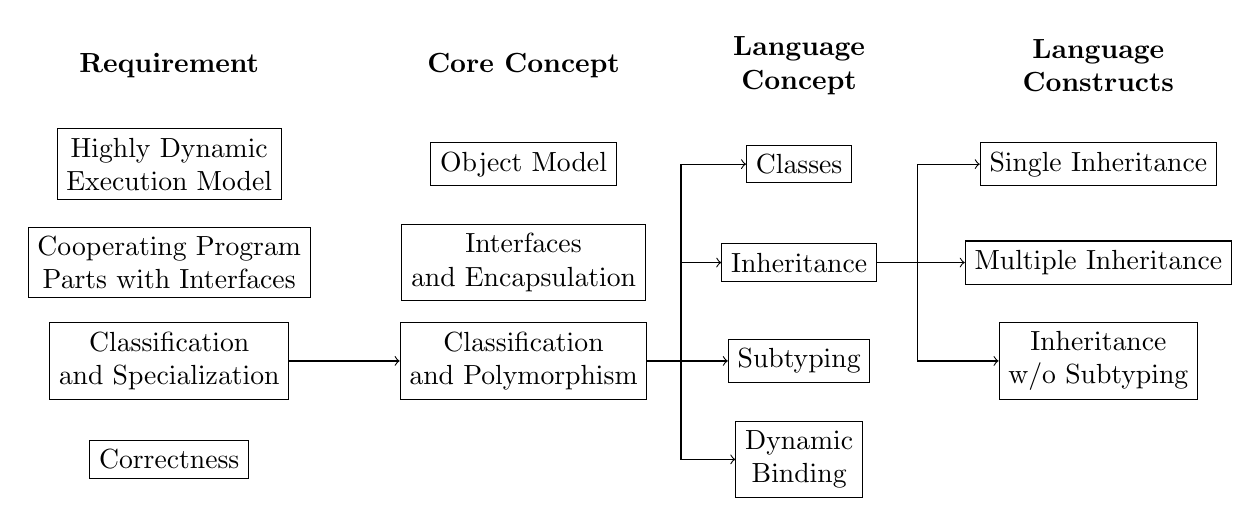
\begin{tikzpicture}
\node [draw, align=center] at (0,0) {Correctness};
\node (a) [draw, align=center] at (0,1.25) {Classification \\ and Specialization};
\node [draw, align=center] at (0,2.5) {Cooperating Program \\ Parts with Interfaces};
\node [draw, align=center] at (0,3.75) {Highly Dynamic \\ Execution Model};

\node (b) [draw, align=center] at (4.5,1.25) {Classification \\ and Polymorphism};
\node [draw, align=center] at (4.5,2.5) {Interfaces \\ and Encapsulation};
\node [draw, align=center] at (4.5,3.75) {Object Model};

\node (c) [draw, align=center] at (8,0) {Dynamic \\ Binding};
\node (d) [draw, align=center] at (8,1.25) {Subtyping};
\node (e) [draw, align=center] at (8,2.5) {Inheritance};
\node (f) [draw, align=center] at (8,3.75) {Classes};

\node (g) [draw, align=center] at (11.8,1.25) {Inheritance \\ w/o Subtyping};
\node (h) [draw, align=center] at (11.8,2.5) {Multiple Inheritance};
\node (i) [draw, align=center] at (11.8,3.75) {Single Inheritance};

\draw [->](a) -- (b);
\draw [->](b) -- (6.5, 1.25) -- (6.5, 0) -- (c);
\draw [->](b) -- (d);
\draw [->](b) -- (6.5, 1.25) -- (6.5, 2.5) -- (e);
\draw [->](b) -- (6.5, 1.25) -- (6.5, 3.75) -- (f);

\draw [->](e) -- (9.5, 2.5) -- (9.5, 1.25) -- (g);
\draw [->](e) -- (h);
\draw [->](e) -- (9.5, 2.5) -- (9.5, 3.75) -- (i);

\node [align = center] at (0, 5) {\textbf{Requirement}};
\node [align = center] at (4.5, 5) {\textbf{Core Concept}};
\node [align = center] at (8, 5) {\textbf{Language} \\ \textbf{Concept}};
\node [align = center] at (11.8, 5) {\textbf{Language} \\ \textbf{Constructs}};
\end{tikzpicture}

\subsection{Language Design Goals}
\begin{mytitle}[Simplicity] Simplicity: Syntax and semantics can easily be understood by users and implementers of the language. Examples: Basic, Pascal, C
\end{mytitle}
\begin{mytitle}[Expressiveness] Language can easily express complex processes and structures. Examples: C\#, Scala, Python
\begin{itemize}
    \item Expressiveness vs. Simplicity: e.g C++ Inheritance, Reflections, yield in Python
\end{itemize}
\end{mytitle}
\begin{mytitle}[Static Safety] Language discourages errors and allows errors to be discovered and reported, ideally at compile time. Examples: Java, C\#, Scala. 
\begin{itemize}
    \item Safety vs. Expressiveness: e.g. static safety says it's wrong if it isn't sure
\end{itemize}
\end{mytitle}
\begin{mytitle}[Modularity] Language allows modules to be compiled separately. Examples: Java, C\#, Scala
\begin{itemize}
    \item Modularity vs. Expressiveness: e.g. automatic types would be great, but one would need to know the whole program
\end{itemize}
\end{mytitle}
\begin{mytitle}[Performance] Programs written in the language can be executed efficiently. Examples: C, C++, Fortran
\begin{itemize}
    \item Performance vs. Simplicity: e.g. memory models give compiler more optimization possibilities, but they are hugely complicated.
    \item Performance vs. Safety: e.g. array bound checks in Java, null pointer checks, garbage collectors
    \item Performance vs. Modularity: e.g. if one knows the whole program, one can optimize lots
\end{itemize}
\end{mytitle}
\begin{mytitle}[Productivity] Language leads to low costs of writing programs. Examples: Visual Basic, Python
\begin{itemize}
    \item Productivity vs. Static Safety: e.g. types give safety but slow down code writing
    \item Productivity vs. Performance: e.g. static types give more performance but less productivity, more performance when going nearer to the hardware but Assembly is just hard to write
\end{itemize}
\end{mytitle}
\begin{mytitle}[Backwards Compatibility] Newer language versions work and interface with programs in older versions. Examples: Java, C (not Python, Scala)
\begin{itemize}
    \item Backwards Compatibility vs. Simplicity: e.g. keep features not used anymore
    \item Backwards Compatibility vs. Expressiveness: biggest problem, cannot introduce features that would break backwards compatibility
    \item Backwards Compatibility vs. Performance: e.g. have to emulate old behaviour
\end{itemize}
\end{mytitle}
